\documentclass[]{article}
\usepackage{float}
\usepackage{graphicx}
\usepackage[svgnames]{xcolor} 
\usepackage{fancyhdr}
\usepackage{fancyvrb}
\usepackage{forest}
\usepackage{tocloft}
\usepackage[hidelinks]{hyperref}
\usepackage{enumitem}
\usepackage[many]{tcolorbox}
\usepackage{listings }
\usepackage[a4paper, total={6in, 8in} , top = 2cm,bottom = 4cm]{geometry}
%\usepackage[a4paper, total={6in, 8in}]{geometry}
\usepackage{afterpage}
\usepackage{amssymb}
\usepackage{pdflscape}
\usepackage{textcomp}
\usepackage{xecolor}
\usepackage{rotating}
\usepackage[Kashida]{xepersian}
\usepackage[T1]{fontenc}
\usepackage{tikz}
\usepackage[utf8]{inputenc}
\usepackage{PTSerif} 
\usepackage{seqsplit}
\usepackage{changepage}


\usepackage{listings}
\usepackage{xcolor}
\usepackage{sectsty}

\setcounter{secnumdepth}{0}
 
\definecolor{codegreen}{rgb}{0,0.6,0}
\definecolor{codegray}{rgb}{0.5,0.5,0.5}
\definecolor{codepurple}{rgb}{0.58,0,0.82}
\definecolor{backcolour}{rgb}{0.95,0.95,0.92}
\definecolor{blanchedalmond}{rgb}{1.0, 0.92, 0.8}
\definecolor{brilliantlavender}{rgb}{0.96, 0.73, 1.0}
 
\NewDocumentCommand{\codeword}{v}{
\texttt{\textcolor{blue}{#1}}
}
\lstset{language=java,keywordstyle={\bfseries \color{blue}}}

\lstdefinestyle{mystyle}{
    backgroundcolor=\color{backcolour},   
    commentstyle=\color{codegreen},
    keywordstyle=\color{magenta},
    numberstyle=\tiny\color{codegray},
    stringstyle=\color{codepurple},
    basicstyle=\ttfamily\normalsize,
    breakatwhitespace=false,         
    breaklines=true,                 
    captionpos=b,                    
    keepspaces=true,                 
    numbers=left,                    
    numbersep=5pt,                  
    showspaces=false,                
    showstringspaces=false,
    showtabs=false,                  
    tabsize=2
}

\lstset{style=mystyle}

\settextfont[BoldFont={XB Zar bold.ttf}]{XB Zar.ttf}

\setlatintextfont[Scale=1.0,
 BoldFont={LiberationSerif-Bold.ttf}, 
 ItalicFont={LiberationSerif-Italic.ttf}]{LiberationSerif-Regular.ttf}


\newfontfamily{\mymono}{[JetBrainsMono-Medium.ttf]}


\newcommand{\inputsample}[1]{
    ~\\
    \textbf{ورودی نمونه}
    ~\\
    \begin{tcolorbox}[breakable,boxrule=0pt]
        \begin{latin}
            \large{
                #1
            }
        \end{latin}
    \end{tcolorbox}
}

\newcommand{\outputsample}[1]{
    ~\\
    \textbf{خروجی نمونه}

    \begin{tcolorbox}[breakable,boxrule=0pt]
        \begin{latin}
            \large{
                #1
            }
        \end{latin}
    \end{tcolorbox}
}
\newcommand{\ybox}[2]{
    \begin{mybox}[colback=yellow]{#1}
	\begin{latin}
            #2
        \end{latin}
    \end{mybox}
}

\newtcolorbox{mybox}[2][]{colback=red!5!white,
colframe=red!75!black,fonttitle=\bfseries,
colbacktitle=red!85!black,enhanced,
attach boxed title to top center={yshift=-2mm},
title=#2,#1}

\newenvironment{changemargin}[2]{%
\begin{list}{}{%
\setlength{\topsep}{0pt}%
\setlength{\leftmargin}{#1}%
\setlength{\rightmargin}{#2}%
\setlength{\listparindent}{\parindent}%
\setlength{\itemindent}{\parindent}%
\setlength{\parsep}{\parskip}%
}%
\item[]}{\end{list}}


\definecolor{foldercolor}{RGB}{124,166,198}
\definecolor{sectionColor}{HTML}{ff5e0e}
\definecolor{subsectionColor}{HTML}{008575}

\definecolor{listColor}{HTML}{00d3b9}

\definecolor{umlrelcolor}{HTML}{3c78d8}

\definecolor{subsubsectionColor}{HTML}{3c78d8}

\defpersianfont\authorFont[Scale=0.9]{XB Zar bold.ttf}

\defpersianfont\titr[Scale=1.5]{Lalezar-Regular.ttf}

\defpersianfont\fehrest[Scale=1.2]{Lalezar-Regular.ttf}

\defpersianfont\fehrestTitle[Scale=3.0]{Lalezar-Regular.ttf}

\defpersianfont\fehrestContent[Scale=1.2]{XB Zar bold.ttf}

\sectionfont{\color{sectionColor}}  % sets colour of sections
\subsectionfont{\color{subsectionColor}}  % sets colour of sections
\subsubsectionfont{\color{subsubsectionColor}}


\renewcommand{\labelitemii}{$\circ$}


\renewcommand{\baselinestretch}{1.1}


\renewcommand{\contentsname}{فهرست}

\renewcommand{\cfttoctitlefont}{\fehrestTitle}


\renewcommand\cftsecfont{\color{sectionColor}\fehrestContent\selectfont}
\renewcommand\cftsubsecfont{\color{subsectionColor}\fehrestContent\selectfont}
\renewcommand\cftsubsubsecfont{\color{subsubsectionColor}\fehrestContent\selectfont}
%\renewcommand{\cftsecpagefont}{\color{sectionColor}}


\setlength{\parskip}{1.2pt}

\begin{document}


%%% title pages
\begin{titlepage}
\begin{center}

\textbf{ \Huge{به نام خدا} }
        
\vspace{0.2cm}


\includegraphics[width=0.4\textwidth]{sharif1.png}\\
\vspace{0.2cm}
\textbf{ \Huge{\emph درس مبانی برنامه‌سازی} }\\
\vspace{0.25cm}
\textbf{ \Large{ فاز دوم پروژه} }
\vspace{0.2cm}
       
 
      \large \textbf{دانشکده مهندسی کامپیوتر}\\\vspace{0.1cm}
    \large   دانشگاه صنعتی شریف\\\vspace{0.2cm}
       \large   ﻧﯿﻢ سال اول 02-01 \\\vspace{0.10cm}
      \noindent\rule[1ex]{\linewidth}{1pt}
استاد:\\
    \textbf{{دکتر محمدامین فضلی}}



    \vspace{0.20cm}

   مهلت ارسال:\\
    \textbf{{فاز دوم: ۱۲ بهمن}}\\
    \textbf{{ساعت 23:59:59}}

    \vspace{0.10cm}
مسئول پروژه:\\
    \textbf{\authorFont{امیرمهدی کوششی}}
    
        \vspace{0.10cm}
مسئول فاز دوم:\\
    \textbf{\authorFont{آرمان بابائی}}
    
        \vspace{0.10cm}
طراحان فاز دوم:\\
    \textbf{\authorFont{محمدمهدی قیدی، سروش شرافت، عرفان مجیبی، زهرا رحمانی، محمد ایزدی، محمد خلفی}}
    
        \vspace{0.05cm}
مسئولین تنظیم مستند:\\
    \textbf{\authorFont{امیرمهدی کوششی، آرمان بابایی}}
    

\end{center}
\end{titlepage}
%%% title pages


%%% header of pages
\newpage
\pagestyle{fancy}
\fancyhf{}
\fancyfoot{}
\cfoot{\thepage}
\lhead{فاز دوم}
\rhead{
\includegraphics[width=0.1\textwidth]{sharif.png}\\
دانشکده مهندسی کامپیوتر
}
\chead{پروژه مبانی برنامه‌سازی}
%%% header of pages
\renewcommand{\headrulewidth}{2pt}
\KashidaOff
\tableofcontents
\newpage
 \Large \textbf{\\\\
}


\section*{{\titr نکات قابل توجه}}
\addcontentsline{toc}{section}{{\fehrestContent نکات قابل توجه}}
\begin{itemize}
\item
پس از اتمام این فاز، در گیت خود یک تگ با ورژن \lr{"v2.0.0"} بزنید. در روز تحویل حضوری این tag بررسی خواهد شد و کدهای پس از آن نمره‌ای نخواهد گرفت. برای اطلاعات بیش‌تر در مورد شیوه ورژن‌گذاری، می‌توانید به
 \href{https://semver.org/}{\textcolor{blue}{\underline{این لینک}}}
 مراجعه کنید. البته برای این پروژه صرفا رعایت کردن همان ورژن گفته شده کافیست، اما خوب‌ است که با منطق ورژن‌بندی هم آشنا بشوید.

\item
در صورت کشف تقلب، برای بار اول منفی نمرهٔ آن فاز برای آن فرد ثبت می‌شود و برای بار دوم، نمرهٔ منفی کل پروژه برای فرد لحاظ خواهد‌ شد.

\end{itemize}

\newpage
\section*{{\titr مقدمه}}
\addcontentsline{toc}{section}{{\fehrestContent مقدمه}}

\subsection*{{\titr اهداف پروژه}}

\addcontentsline{toc}{subsection}{{\fehrestContent اهداف قابل توجه}}

\begin{itemize}

\item
هدف این پروژه طراحی یک ابزار ویرایش فایل مشابه vim است. احتمالا در کارگاه کامپیوتر و یا جاهای دیگر با این ابزار کار کرده‌اید. در غیر این صورت می‌توانید از طریق \href{https://www.openvim.com}{\textcolor{blue}{\underline{این لینک}}} نحوه کار با این ابزار را ببینید.

\item
در این فاز از برای ابزاری که در فاز قبل طراحی کردید رابط کاربری می‌سازید و برخی ویژگی‌ها را بهبود می‌دهید.

\item
در این پروژه نحوه پیاده‌سازی اجزای مختلف از اهمیت بسیاری برخوردار است و تنها خروجی نهایی مهم نیست. از این رو برای تمیزی کد خود ارزش قائل شوید. 

\item
آشنایی با سیستم مدیریت نسخه \lr{Git} و کار بر روی پروژه بر بستر یک مخزن \lr{Github}، یکی از اهداف مهم پروژه است. در این مورد توصیه می‌شود تغییرات خود را در دوره‌های کوتاه مدت \lr{commit} کنید.

\end{itemize}

\subsection*{{\titr کلیات پروژه}}
\addcontentsline{toc}{subsection}{{\fehrestContent کلیات پروژه}}

در این فاز، کد فاز اول خود را کامل می‌کنید.

در ادامهٔ مستند، موجودیت‌ها، نمای کلی رابط کاربری سیستم، نقش‌ها و دستورات لازم شرح داده‌شده است.

\begin{enumerate}[label={نکته \arabic*:}]
\item
در هر جایی از پروژه می‌توانید هرگونه خلاقیتی را به‌کار ببرید. با این حال توجه کنید که خواسته‌های واضح پروژه بایستی انجام شوند و سیستم ورودی گرفتن و خروجی دادن شما باید مطابق جزییات گفته شده در این مستند باشد.


\item در این فاز برخی از دستورات را با استفاده کلیدهای شورتکات پیاده‌سازی می‌کنید. کلیدهای ذکرشده در ادامه‌ی مستند پیشنهادی هستند و می‌توانید به صلاح‌دید خود آن‌ها را تغییر دهید. توجه کنید که این کار نباید منجر به محدود شدن کاربری برنامه‌ی شما شود.
% \newpage
% \item
% در مستند بعضی از دستور‌هایی که مشاهده می‌کنید فرمتی به شکل زیر دارند:

% \begin{mybox}[colback=yellow]{دستور}
	
	
% 	\begin{latin}
		
% 	compare file1 file2
		
% 	\end{latin}
	
% \end{mybox}
% همچنین توجه کنید که اگر دستور نامعتبری وارد شد که در قسمت مربوطه، برای آن خطای به خصوصی در نظر گرفته نشده بود، پیام زیر را چاپ کنید:

% \begin{mybox}[colback=yellow]{پیغام به کاربر}
	
	
% 	\begin{latin}
		
% 	invalid command
		
% 	\end{latin}
	
% \end{mybox}


\end{enumerate}

\newpage
\section*{{\titr معرفی ابزار}}
\addcontentsline{toc}{section}{{\fehrestContent معرفی ابزار}}
همانطور که قبلا توضیح دادیم، شما باید یک ابزار ویرایش متن مانند vim طراحی کنید. در این فاز از پروژه، شما باید یک محیط گرافیکی مانند خود vim بالا بیاورید و تمامی دستوراتی که به برنامه خود می‌دهید از طریق همین محیط گرافیکی است. شما باید از طریق محیط گرافیکی دستورات را بگیرید و پردازش کنید و تغییرات را روی فایل‌ها اعمال کنید و در نهایت خروجی مناسب را به صورت زنده (live) به کاربر نمایش دهید.
\newpage
\section*{{\titr توضیح بخش‌های مختلف پروژه}}
\addcontentsline{toc}{section}{{\fehrestContent توضیح بخش‌های مختلف پروژه}}

\subsection*{{\titr موارد عمومی و قابلیت‌های ابزار}}
\addcontentsline{toc}{subsection}{{\fehrestContent موارد عمومی و قابلیت‌های ابزار}}


در این فاز بنابر این داریم تا رابط گرافیکی یا GUI مربوط به فاز اول را پیاده‌سازی نماییم. در فاز اول مواردی پیاده‌سازی کردید که با ترمینال انجام دادید و در این فاز موارد گرافیکی مربوط به vim را خواهیم نوشت.


\subsubsection*{{\titr Layout Window}}
\addcontentsline{toc}{subsubsection}{{\fehrestContent Layout Window}}

برای نشان دادن مواردی که کاربر تایپ می‌کند و محتویات فایل مورد بررسی نیاز داریم تا یک پنجره داشته باشیم تا پایه‌ریزی کلی یا layout مواردی که قرار است نشان داده شوند را در آن به نمایش بگذاریم. یک پنجره vim به طور کلی باید قادر به نمایش ۵ بخش زیر باشد که به همراه تطابق آن‌ها با تصویر آمده‌اند:

\begin{itemize}
    \item اسم فایل و وضعیت ذخیره شدن آن در دیسک (ذخیره شده/نشده)\\
    اسم فایل روبروی کلمه‌ی NORMAL آمده است. ذخیره‌نشده بودن فایل با استفاده از علامت + در کنار اسم فایل نشان داده شده است.
    \item حالت فعلی vim یا mode\\
    کلمه‌ی NORMAL در تصویر به این کار اختصاص داده شده.
    \item خط دستور یا command bar که دستوراتی که در ادامه داک می‌آیند در این قسمت وارد می‌شوند.\\
    این قسمت در آخرین خط صفحه آمده است. با زدن کلید / و یا : در حالت NORMAL کاربر شروع به تایپ در این محدوده می‌کند و تا زمانی که کلید enter را فشار نداده به این کار ادامه می‌دهد.
    \item شماره هر خط فایل\\
    این شماره‌ها در سمت چپ خطوط نوشته شده‌اند.
    \item و در نهایت محتویات فایل
\end{itemize}

ادیتور vim به صورت کلی ۳ حالت اصلی insert و normal و visual را دارد. در هر کدام از این حالت‌ها کارهای بخصوصی می‌توان انجام داد که در ادامه داک و برای هر دستور ذکر شده است که باید در کدام حالت اعمال شوند. برای گرفتن شهود بیشتر م‌یتوانید عکس زیر را مشاهده کنید که می‌تواند پیاده‌سازی مطلوبی از موارد بالا باشد.

\begin{figure}[H]
    \centerline{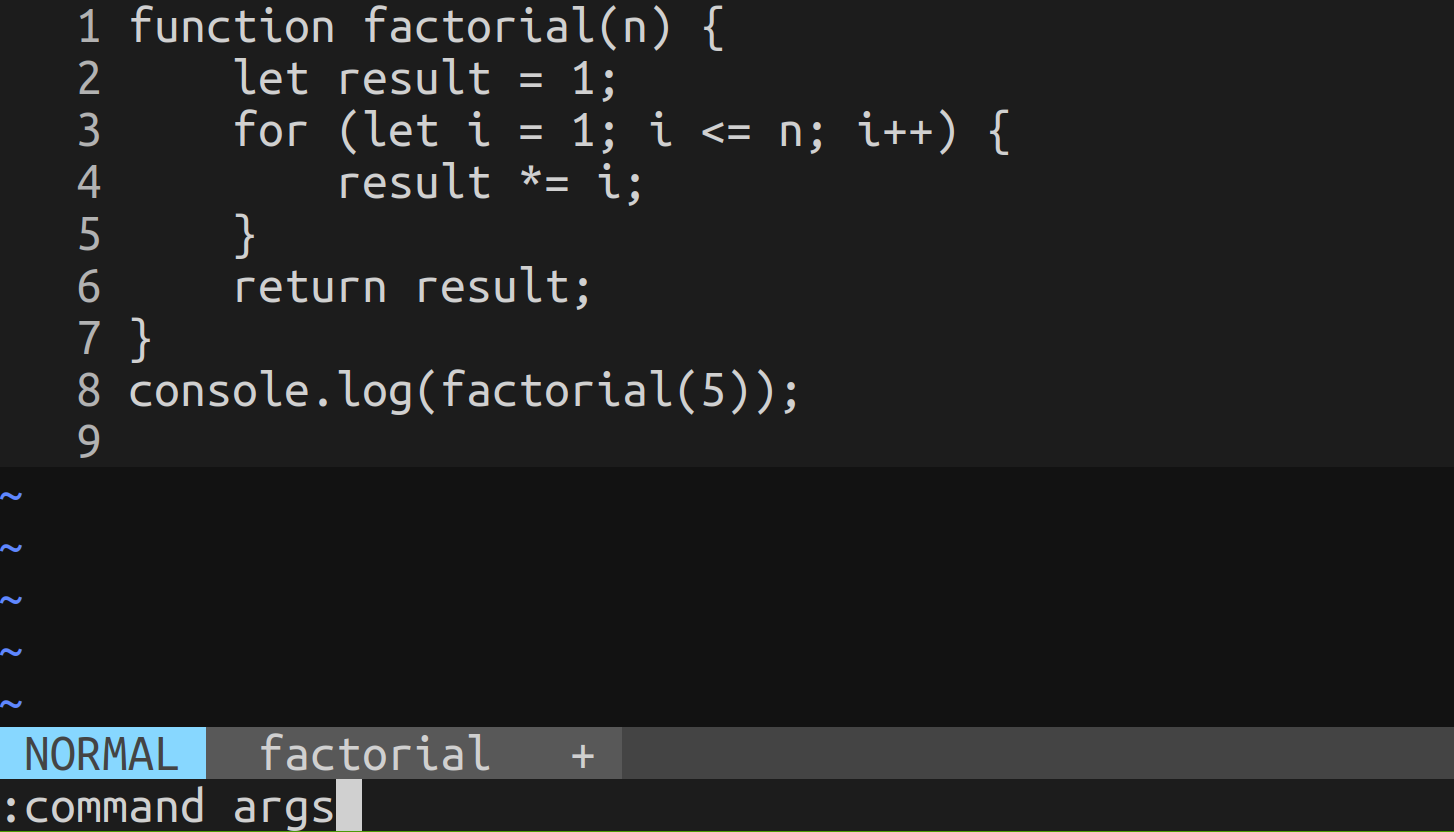
\includegraphics[width=\textwidth]{Resources/window_layout.png}}
\end{figure}


\subsubsection*{{\titr Navigation}}
\addcontentsline{toc}{subsubsection}{{\fehrestContent Navigation}}

برنامه‌ی شما باید قابلیت حرکت دادن نشان‌گر (cursor) با استفاده از کیبورد بر روی متون را داشته باشد. مواردی که باید پیاده سازی به آنها توجه کنید:
\begin{itemize}
    \item کاربر باید بتواند نشان‌گر (cursor) را بر روی بخشی از متن که در حال نمایش است به چپ و راست و بالا و پایین حرکت دهد. (کلیدهای پیشنهادی: بالا(k) پایین(j) چپ(h) و راست(l))
    \item با رسیدن به ابتدای هر خط، با فشردن کلید چپ و همچنین با رسیدن به انتها خط و فشردن کلید راست، نباید اتفاقی بیفتد.
    \item انتقال به خط بعد/قبل (بالا و پایین رفتن) باید به مکان نسبی مشابه مکان نسبی نشان‌گر (cursor) در خط فعلی باشد. (برای مثال اگر در خط فعلی در کاراکتر بیستم قرار داریم، با فشردن کلید j باید در خط بعد و    کاراکتر بیستم قرار داشته باشیم.) اگر تعداد کاراکتر خط بعدی کمتر بود، به آخرین کاراکتر آن انتقال یابیم.
    \item در ۴ خط مانده به پایان صفحه فعلی، با فشردن کلید حرکت به پایین، باید یک خط شیفت دهید. یعنی یک خط جدید از فایل به صفحه اضافه شده و خط اول حذف شود. همچنین وقتی نشان‌گر (cursor) در محل ۴ خط مانده به ابتدای صفحه فعلی است، در صورت فشردن کلید بالا، باید یک خط از بالای صفحه اضافه شده و یک خط از پایین حذف شود.
    \item لازم است توجه کنید با کلید پایین رفتن باید به خط بعدی با توجه کاراکتر \textbackslash n بروید و شکل ظاهری خطوط ملاک نیست.
\end{itemize}

\subsubsection*{{\titr Selection}}
\addcontentsline{toc}{subsubsection}{{\fehrestContent Selection}}


در حالت بصری یا همان visual امکان این را داریم که قسمتی از محتویات فایل را انتخاب (select) کرده و با آن قسمت انتخاب شده مواردی چون copy یا cut یا delete را بتوانیم انجام دهیم.
در پیاده‌سازی شما از محل نشان‌گر (cursor) در زمان ورود به حالت visual تا محل فعلی نشان‌گر (cursor) باید انتخاب شود. می‌توانید این انتخاب را با هایلایت کردن قسمت انتخاب‌شده نشان دهید.

توجه کنید که در حالت بصری همچنان قابلیت جابجا کردن نشان‌گر (cursor) وجود دارد و این حرکت می‌تواند به سمت بعد یا قبل (و یا ترکیبی از این دو) محل aنشان‌گر (cursor) در هنگام ورود به حالت بصری باشد.


\subsubsection*{{\titr Clipboard}}
\addcontentsline{toc}{subsubsection}{{\fehrestContent Clipboard}}


پس از انتخاب قسمتی از متن در حالت
visual
باید این امکان برای کاربر وجود داشته باشد که متن انتخاب شده را حذف، قیچی و یا روگرفت بکند. کاربر باید بتواند در حالتی که متن انتخاب شده، به وسیله هر کدام از دستورات زیر عملیات مورد نظر خودش را انجام بدهد.

\begin{latin}
    \begin{itemize}
        \item{Cut/Delete}: d
        \item{Copy}: y
    \end{itemize}
\end{latin}

بدین منظور باید یک فیچر clipboard برای ادیتور خود پیاده‌سازی کنید تا قسمت‌هایی که cut/copy می‌شوند در آن قرار بگیرند. پس از هر کدام از کلیدهای مربوط به روگرفت و یا قیچی باید از حالت visual به حالت normal منتقل شوید.
توجه کنید که دستورات قیچی و روگرفت فاز اول هم در همین دسته محسوب می‌شوند و فرقی نمی‌کند که از کلیدها و یا دستورات فاز اول برای اضافه کردن متن به clipboard استفاده شده باشد.

دستور paste که در حالت normal تعریف می‌شود
به کاربر این امکان را می‌دهد که در این حالت بتواند به وسیله کلید p مقدار ذخیره‌شده در clipboard برنامه (که حاصل اجرای یک دستور cut یا copy بوده است) را در محل نشان‌گر (cursor) قرار دهد.

\newpage

\subsubsection*{{\titr Saving}}
\addcontentsline{toc}{subsubsection}{{\fehrestContent Saving}}


برنامه شما باید به کاربر این امکان را بدهد که با زدن کامند 
\ybox{دستور}{:save}
فایل فعلی خود را ذخیره کند. در صورتی که کاربر قبلاً برای فایل خود اسم انتخاب نکرده باشد باید با چاپ پیام مناسب (احتمالا در محل ورودی گرفتن دستور) از او بخواهید برای فایل خود اسم انتخاب کند.
همچنین با زدن کامند

\ybox{دستور}{:saveas <name>}

کاربر باید بتواند فایل را با نام دلخواهش ذخیره کند.
پس از تکمیل فرایند ذخیره نیز با نمایش پیام مناسب موفقیت‌آمیز بودن ذخیره را به کاربر اطلاع دهید.

\subsubsection*{{\titr Open}}
\addcontentsline{toc}{subsubsection}{{\fehrestContent Open}}


در این فاز باید امکان باز کردن یک فایل جدید در برنامه را پیاده سازی کنید. با وارد کردن این کامند باید یک فایل جدید در ویرایشگر باز شود. اگر از قبل فایلی باز بوده، محتوای آن باید سیو شود و بسته شود و فایل جدید جایگزین آن شود.

\ybox{دستور}{:open <file>}

\subsubsection*{{\titr Undo}}
\addcontentsline{toc}{subsubsection}{{\fehrestContent Undo}}


این امکان را در فاز قبل پیاده سازی کرده‌اید و باید یک شورتکات هم برای آن تعریف کنید. شورتکات پیشنهادی کلید u در حالت نرمال است. بنابراین کاربر حداقل به دو صورت امکان undo داشته باشد:
\begin{itemize}
    \item زدن دکمه u در حالت نرمال
    \item زدن کامند :undo
\end{itemize}

\newpage
\subsubsection*{{\titr Find}}
\addcontentsline{toc}{subsubsection}{{\fehrestContent Find}}


با وارد کردن کامند

\ybox{دستور}{/<expression>}

باید همه‌ی رخدادهای <expression> را در متن پیدا و آن ها highlight کنید.
همچنان باید این قابلیت را پیاده سازی کنید که با استفاده از کلید ،n نشان‌گر (cursor) به اولین مکان رخداد <expression> پس از مکان فعلی نشان‌گر (cursor) برود. (اگر چنین رخدادی وجود نداشت نشان‌گر (cursor) باید  به اولین رخداد برود و اگر هیچ رخدادی وجود نداشت مکان نشان‌گر (cursor) نباید تغییر کند)
دقت کنید که پس وارد کردن هر کلید یا کامندی به جز کلید n باید هایلایت‌های مربوط به کامند find را پاک کنید.

\subsubsection*{{\titr Replace}}
\addcontentsline{toc}{subsubsection}{{\fehrestContent Replace}}

دستور replace با تغییر اندک مشابه فاز اول باقی می‌ماند. در صورتی که نام فایل در دستور آمده بود 
(منظور همان آرگومان -file است)
با این دستور مشابه دستورات دیگر فاز اول برخورد کنید، اما در صورتی که آرگومان -file در دستور وجود نداشت عملیات را در فایلی که در ویرایشگر باز است انجام دهید. علاوه بر این در صورتی که تغییری در فایل ایجاد شد، نشان‌گر (cursor) را به موقعیت شروع اولین تغییر انتقال دهید.

\ybox{مثال}{:replace --str1 "salam khubi?" --str2 "Dorud! Che Khabar?" -at 2}

در نتیجه‌ی این دستور باید دومین مقدار رشته‌ی str1 در فایل با str2 جابجا شود و نشان‌گر (cursor) به جایی که دومین str1 در آن قرار داشت، منتقل شود.
\subsubsection*{{\titr Auto-indent}}
\addcontentsline{toc}{subsubsection}{{\fehrestContent Auto-indent}}


این دستور را در فاز یک پیاده سازی کرده‌اید. در این فاز باید علاوه بر در نظر گرفتن کامند auto-indent برای اجرای این دستور، یک shortcut نیز برای آن تعریف کنید. کلید پیشنهادی برای این منظور کلید = است. واضح است که تعریف این کلید در حالت normal کافی‌ست.
\subsubsection*{{\titr دستورات فاز اول}}
\addcontentsline{toc}{subsubsection}{{\fehrestContent دستورات فاز اول}}


این فاز هیچ کدام از دستورات فاز اول را منسوخ نمی‌کند؛ به این معنی که تمام دستورهایی که در فاز قبل وجود داشتند مثل insertstr یا arman یا... در این فاز هم به همان شکل وجود دارند. حتی دستوری مثل find که در این فاز به نوع جدیدی مطرح شده، باید به صورت فاز اول هم قابل‌استفاده باشد.
تنها تغییری که در این دستورات به وجود می‌آید این است که یک کاراکتر ":" به ابتدای این دستورات اضافه می‌شود.

\ybox{مثال}{:createfile file\_name.txt}

خروجی این دستورات (در صورت وجود) باید به صورت یک فایل بدون نام در ویرایشگر باز شوند. پس مثلا اگر دستور

\ybox{مثال}{:tree}

وارد شد، لازم است فایل فعلی در صورت وجود بسته شود، و یک فایل بدون نام با محتوای درخت مشابه فاز اول باز شود. واضح است که امکان جستجو، تغییر و ذخیره‌سازی مثل هر فایل دیگری برای این فایل هم تعریف شده است. با این وجود در صورتی که این فایل بدون ذخیره‌سازی بسته شد (یا فایل جدیدی باز شد) لازم است هیچ اثری از این فایل باقی نماند.


\end{document}


